\section{Intro}
\begin{frame}{Stars, right?}
    \begin{columns}
        \begin{column}{0.5\textwidth}
        \Large
            \onslide<2->{ 
                They're all around, they provide heat and occasionally, light. \vspace{10pt} \\
                }
            \onslide<3->{
                How? Through nuclear fusion!
            }
        \end{column}
        \begin{column}{0.5\textwidth}
            \onslide<1->{
                \begin{figure}
                    \centering
                    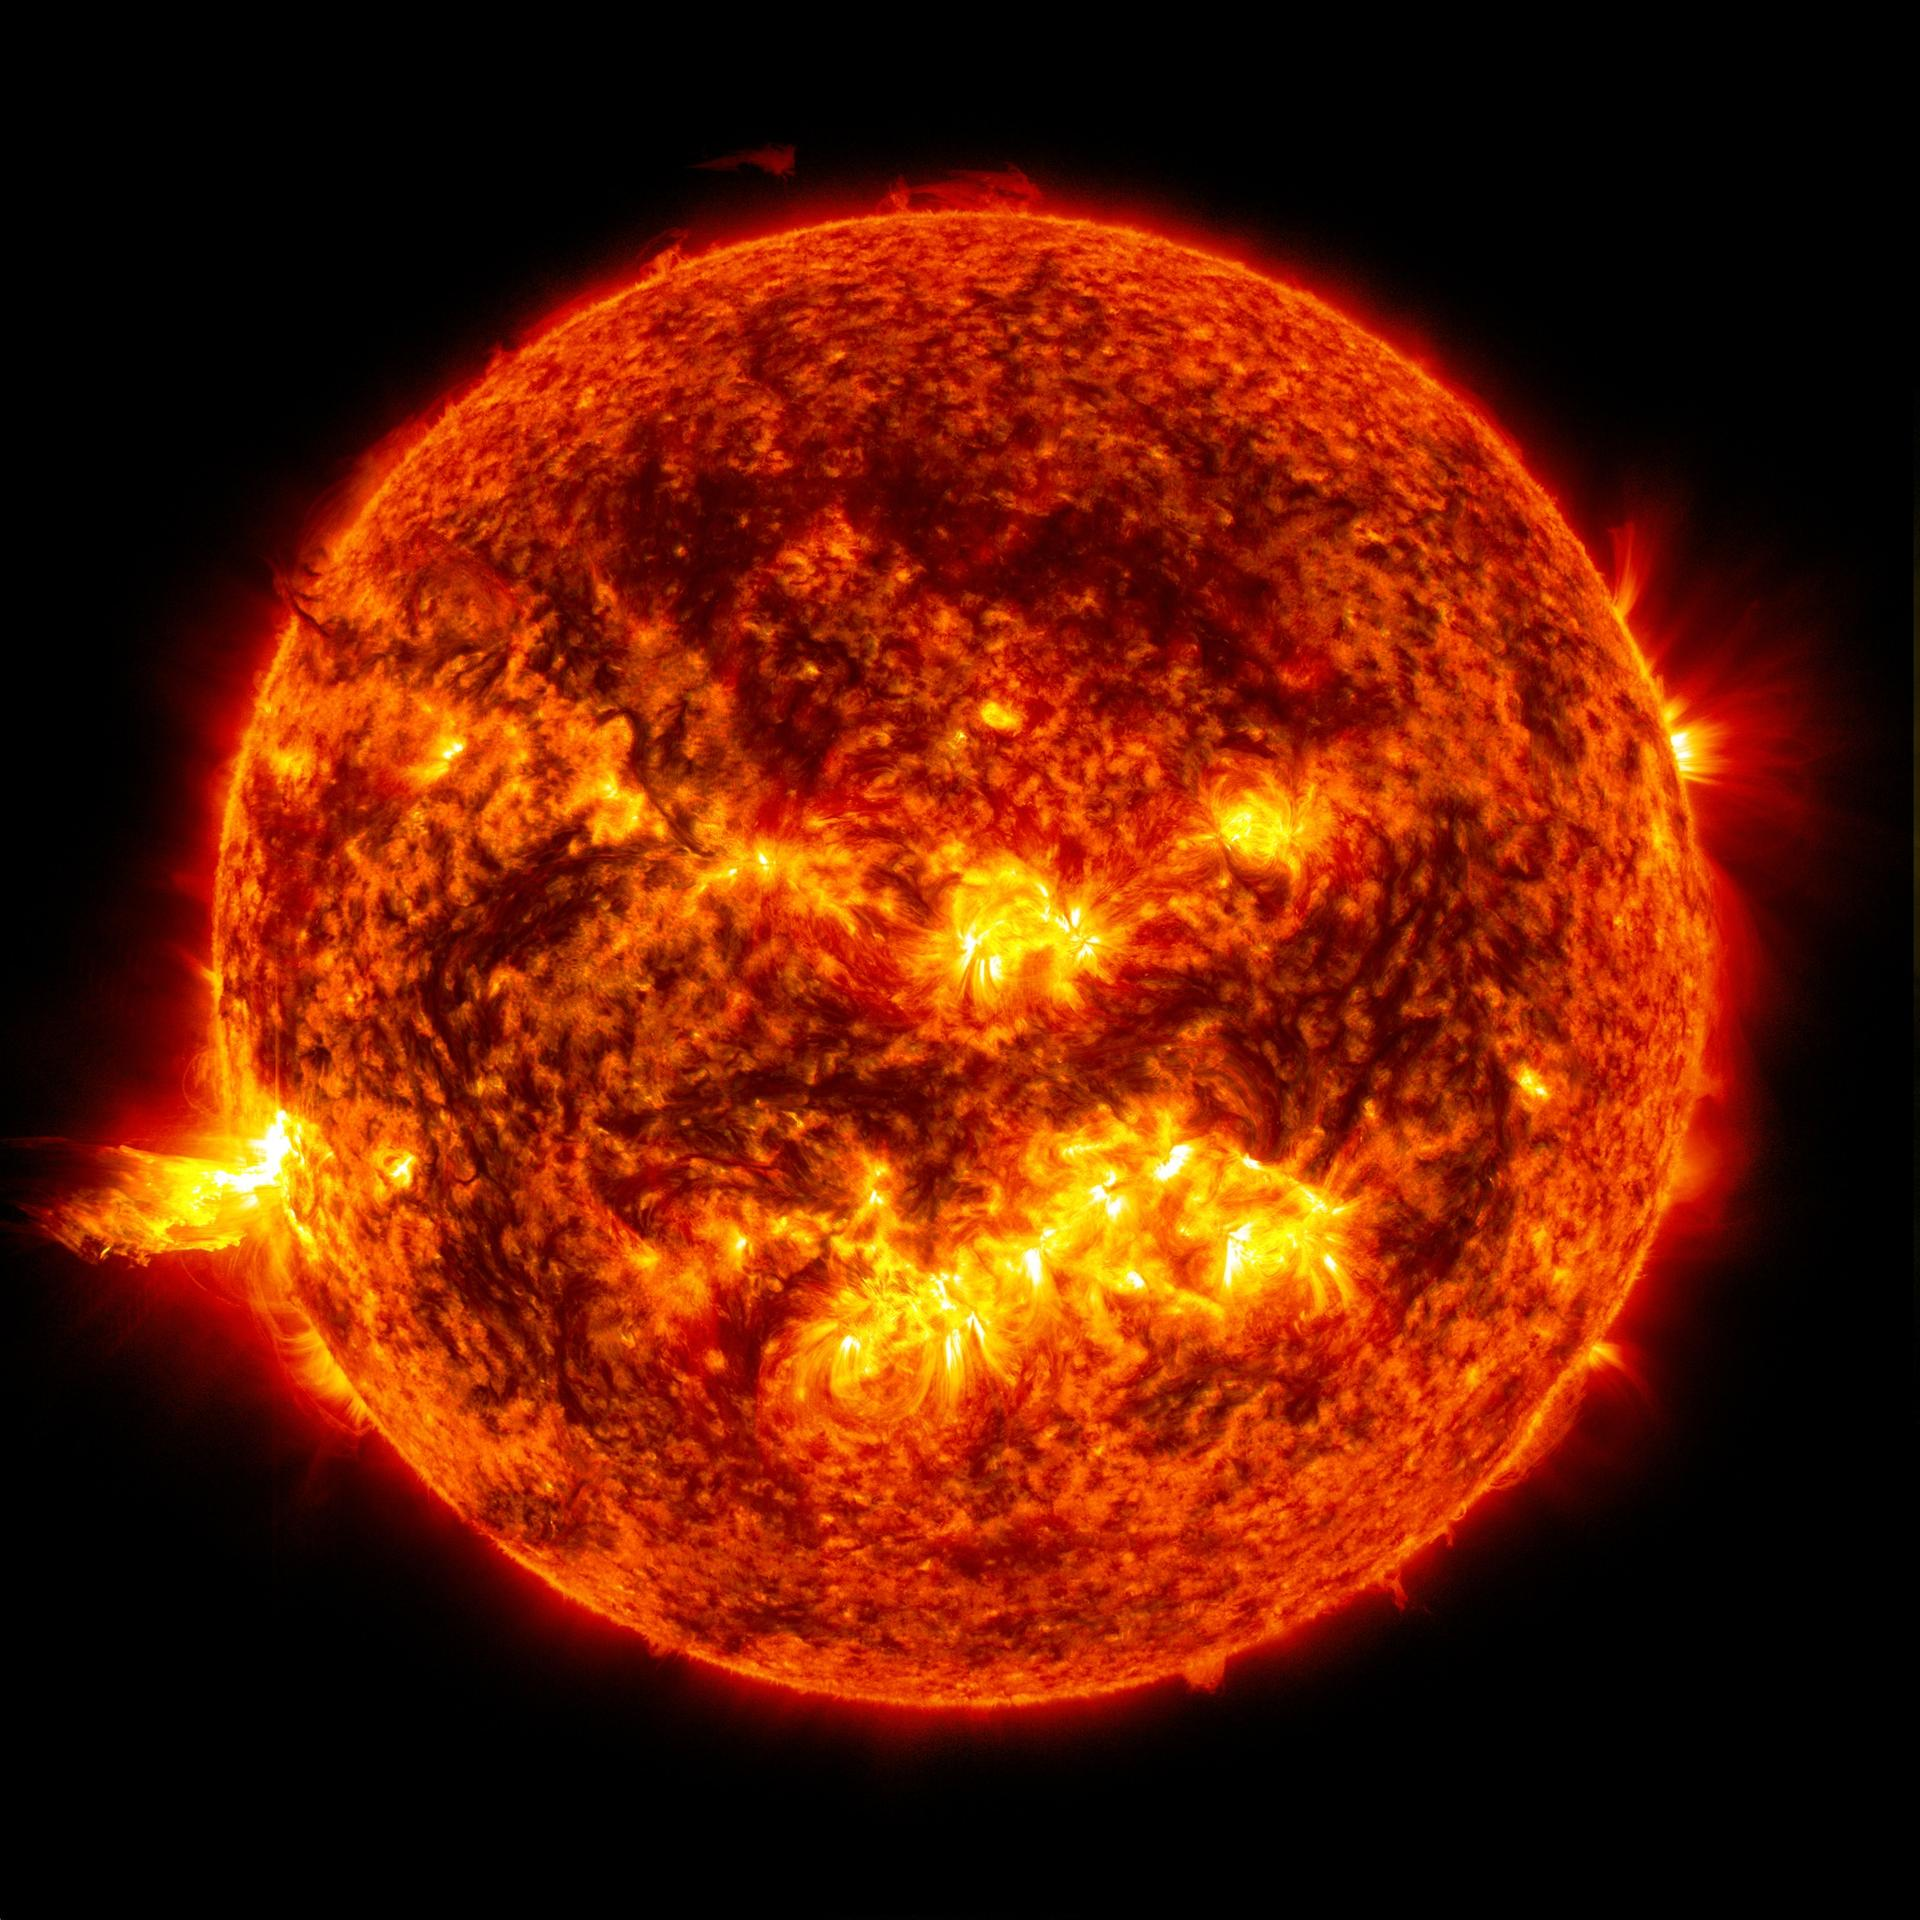
\includegraphics[width = \columnwidth]{figs/sun.jpg}
                    \caption{A close-by star, \\ credit: NASA, GSFC}
                    \label{fig:enter-label}
                \end{figure}
            }    
        \end{column}
    \end{columns}
\end{frame}
\begin{frame}{Thermonuclear Reactions}
\onslide<1-5>{
    \begin{center}
    \Huge
        A + B $\rightarrow$ C
    \end{center}
}
\Large
    \begin{gather*}
    \onslide<1-5>{
        \text{C generation}  = 
        } 
    \begin{array}{c}
        \onslide<2-5>{
            \text{\textcolor{red}{Abundance of A}} \\
        }  
        \onslide<3-5>{
                \text{\textcolor{olive}{Abundance of B}} \\
        } 
        \onslide<4-5>{
                \text{\textcolor{blue}{Reaction Rate}} \\
        }
        \onslide<5-5>{
                \text{\textcolor{orange}{Mass Density}} 
        }
    \end{array}
    \end{gather*}
\end{frame}
\begin{frame}{Hydrogen Fusion}
\onslide<1->{
    \begin{center}
    \Huge
        $^1$H + $^1$ H $\rightarrow$ $^2$H
    \end{center}
}
\Large
    \begin{gather*}
        \onslide<2->{
            \frac{dY_\mathrm{^1H}}{dt}  = -     
            \text{\textcolor{red}{$Y_\mathrm{^1H}$}}
            \text{\textcolor{olive}{$Y_\mathrm{^1H}$}}
            \text{\textcolor{blue}{$\lambda_{^1\mathrm{H} \rightarrow ^2\mathrm{H}}$}} 
            \text{\textcolor{orange}{$\rho$}} 
        }
    \end{gather*}
        \begin{gather*}
        \onslide<3->{
            \frac{dY_\mathrm{^2H}}{dt}  = 
            \text{\textcolor{red}{$Y_\mathrm{^1H}$}}
            \text{\textcolor{olive}{$Y_\mathrm{^1H}$}}
            \text{\textcolor{blue}{$\lambda_{^1\mathrm{H} \rightarrow ^2\mathrm{H}}$}} 
            \text{\textcolor{orange}{$\rho$}} 
        }
    \end{gather*}
\end{frame}
\begin{frame}{Hydrogen Fusion + Deuterium Fusion}
\onslide<1->{
    \begin{align*}
        {}^\text{1}\text{H} + {}^\text{1}\text{H}&\rightarrow {}^\text{2}\text{H}\\
        {}^\text{1}\text{H} + {}^\text{2}\text{H}&\rightarrow {}^\text{3}\text{He}
    \end{align*}
}
\Large
    \begin{gather*}
        \onslide<2->{
            \frac{dY_\mathrm{^1H}}{dt}  = -     
            \text{\textcolor{red}{$Y_\mathrm{^1H}$}}
            \text{\textcolor{olive}{$Y_\mathrm{^1H}$}}
            \text{\textcolor{blue}{$\lambda_1$}} 
            \text{\textcolor{orange}{$\rho$}} 
        }
        \onslide<4->{
            -
            \text{\textcolor{red}{$Y_\mathrm{^1H}$}}
            \text{\textcolor{olive}{$Y_\mathrm{^2H}$}}
            \text{\textcolor{blue}{$\lambda_2$}} 
            \text{\textcolor{orange}{$\rho$}} 
        }
    \end{gather*}
    \begin{gather*}
        \onslide<2->{
            \frac{dY_\mathrm{^2H}}{dt}  = 
            \text{\textcolor{red}{$Y_\mathrm{^1H}$}}
            \text{\textcolor{olive}{$Y_\mathrm{^1H}$}}
            \text{\textcolor{blue}{$\lambda_1$}} 
            \text{\textcolor{orange}{$\rho$}} 
        }
        \onslide<4->{
            -
            \text{\textcolor{red}{$Y_\mathrm{^1H}$}}
            \text{\textcolor{olive}{$Y_\mathrm{^2H}$}}
            \text{\textcolor{blue}{$\lambda_2$}} 
            \text{\textcolor{orange}{$\rho$}} 
        }
    \end{gather*}
    \begin{gather*}
        \onslide<3->{
            \frac{dY_\mathrm{^3He}}{dt}  = 
            \text{\textcolor{red}{$Y_\mathrm{^1H}$}}
            \text{\textcolor{olive}{$Y_\mathrm{^2H}$}}
            \text{\textcolor{blue}{$\lambda_2$}} 
            \text{\textcolor{orange}{$\rho$}} 
        }
    \end{gather*}
\end{frame}
\begin{frame}{pp-chain vs CNO-cycle}
    \Large
        \begin{columns}
        \begin{column}{0.5\textwidth}
            \only<1-2>{
            \begin{align*}
                {}^\text{1}\text{H} + {}^\text{1}\text{H}&\rightarrow {}^\text{2}\text{H}\\
                {}^\text{1}\text{H} + {}^\text{2}\text{H}&\rightarrow {}^\text{3}\text{He}\\
                {}^\text{3}\text{He} + {}^\text{1}\text{H}&\rightarrow {}^\text{4}\text{He}
            \end{align*}
            \normalsize \centering
            4 species $\rightarrow$ 4 diff. equations
            }    
        \end{column}
        \begin{column}{0.5\textwidth}
        \Large
            \only<2>{
            \begin{align*}
                 {}^\text{12}\text{C} + {}^\text{1}\text{H} &\rightarrow {}^\text{13}\text{N}  \\
                 {}^\text{13}\text{N} &\rightarrow {}^\text{13}\text{C} \\
                 {}^\text{13}\text{C} + {}^\text{1}\text{H} &\rightarrow {}^\text{14}\text{N} \\
                 {}^\text{14}\text{N} + {}^\text{1}\text{H} &\rightarrow {}^\text{15}\text{O} \\
                 {}^\text{15}\text{O} &\rightarrow {}^\text{15}\text{N} \\
                 {}^\text{15}\text{N} + {}^\text{1}\text{H} &\rightarrow {}^\text{12}\text{C} + {}^\text{4}\text{He}
            \end{align*}
            \normalsize \centering
            8 species $\rightarrow$ 8 diff. equations
            }
        \end{column}
    \end{columns}
\only<3>{
\begin{figure}
    \centering
    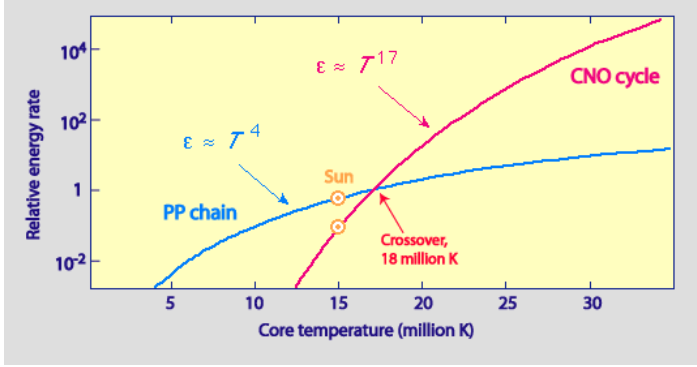
\includegraphics[width = \textwidth]{figs/cross.png}
    \caption{Source: Mike Guidry, University of Tennessee}
    \label{fig:enter-label}
\end{figure}
}
\end{frame}
\begin{frame}{Which one is faster}
\onslide<1->{
    \centering
    Two things control the efficiency \vspace{10pt}
    \begin{columns}
        \begin{column}{0.5\textwidth}
            Core Temperature $\rightarrow$  \textcolor{blue}{Reaction Rate}
        \end{column}
        \begin{column}{0.5\textwidth}
            Metallicity  $\rightarrow$  \textcolor{olive}{Catalyst Abundances}
        \end{column}
    \end{columns}
}
\onslide<2->{
    \vspace{40pt} \Large \centering
    Which is the dominant fusion pathway, as a function of core temperature and metallicity?
}
\end{frame}